\documentclass[polish,polish,a4paper]{article}
\usepackage{cmap}

\usepackage[T1]{fontenc}
\usepackage[utf8]{inputenc}
\usepackage{listings}
\usepackage{graphicx} 
\usepackage{tikz}
\usepackage{xcolor}
\usepackage{babel}
\usepackage{pslatex}
\usepackage{tikz}
\usepackage{pgfplots}
\usepackage{anysize}
\usepackage{pgfgantt}
\usepackage{latexsym,amsmath}

\marginsize{2.5cm}{2.5cm}{3cm}{3cm}
\graphicspath{ {D:\Nauka\Grafika Komputerowa\lab4 światło\latex} }


\title{Sprawozdanie z projektu}
\author{Łukasz Szumilas, Grupa E02-81o}
\date{Zajęcia: 14 stycznia 2018 (odrobione 28 stycznia)}

\begin{document}
  \begin{center}\Large
    Grafika Komputerowa i Komunikacja Człowiek-Komputer
  \end{center}
  \hrule
  {\let\newpage\relax\maketitle}
  \hrule


  \section{Omówienie tematu}
  Celem ćwiczenia było zapoznanie się z elementem HTML5 \textit{canvas}, który użyty był do rysowania grafiki w postaci 2D i 3D przy użyciu skryptów JavaScript.
\\\indent. Po zapoznaniu się z instrukcją na stronie laboratorium, korzystając z odpowiednich funkcji trzeba było narysować czworościan foremny. Najważniejszym elementem było odpowiednie zdefiniowanie punktów w przestrzeni (\textit{triangleVertices}), oraz odpowiednie ich połączenie (\textit{triangleFaces}). Zmienić trzeba było także parametry funkcji \textit{vertexAttribPointer}, mającej za zadanie przypisanie bufora do zmiennych atrybutów koloru i pozycji. W funkcji \textit{drawElements} wpisujemy liczbę elementów figury. Najważniejsze fragmenty kodu i efekt wizualny zawarty jest w \textbf{\textit{kodzie nr 1 i rysunku nr 1}}. 
\\\indent Na zrzucie ekranu widoczne są opcje dotyczące obrotu figury wokół trzech osi, które zostały dodane dzięki instrukcji laboratoryjnej. Problemem było przyspieszanie obrotu figury za każdem naciśnięciem przycisku `Uruchom'. Przycisk ten uruchamiał funkcję \textit{runWebGL()}, która niepotrzebnie za każdym razem inicjalizowała zbyt wiele rzeczy. Po pierwszym uruchomieniu programu, prosta instrukcja warunkowa za każdym kolejnym razem pobierała już tylko funkcję \textit{getRotation}, która wystarczała do odpowiedniego obrotu figury przy stałej prędkości ( \textbf{\textit{kod nr 2}}).
\\\indent Kolejnym etapem było narysowanie fraktalu 2D przy pomocy elementów canvas. Wybraną przeze mnie figurą był trójkąt, który przy pomocy odpowiedniego algorytmu dzielił się na trzy mniejsze trójkąty, zostawiając w środku wycięty odwrócony trójkąt w wymiarach takich samych jak trzy poprzednie. Bazowało to na dywanie Sierpińskiego, gdzie trójkąt zastępuje w samopodziale inną figurę, kwadrat. Manipulując jedynie zmienną \textit{var najwyzszyPoziom}, trójkąt dochodził do coraz to większego samopodziału. Aby urozmaicić wygląd oglądanego obrazka, zostały zastosowane losowe kolory. Odbyło się to za pomocą odpowiednio podzielonego gradientu, gdzie każdy odcinek przechodził w osobnie wylosowane kolory. Trójkąty zostawały także poddawane perturbacjom zgodnie z ustawioną zmienną \textit{var perturbance}. Najważniejsze fragmenty i efekty zostały przedstawione w \textbf{\textit{kodzie nr 3 i rysunku nr 2 i 3}}.
  \section{Omówienie kodu}
   \textbf{Kod 1}, fragmenty realizujące czworościan foremny.
{\small
\begin{lstlisting}[language=C++]
var triangleVertices = [
      1,1,1, //w
      0,0,0,    //c
      -1,1,-1,  //w
      1,0,0,    //c 
      -1,-1,1,   //w
      1,1,0,	//c
      1,-1,-1,	//w
      0,1,0	//c
   ];
   
   var triangleFaces = [
      0,1,2,
      0,2,3,
	  0,1,3,
	  1,2,3
   ];
   
   //fragmenty funkcji gl_draw()
       gl_ctx.vertexAttribPointer(_position, 3, gl_ctx.FLOAT, false, 4*(3+3), 0);
      gl_ctx.vertexAttribPointer(_color, 3, gl_ctx.FLOAT, false, 4*(3+3), 3*4);
   
         gl_ctx.drawElements(gl_ctx.TRIANGLES, 12, gl_ctx.UNSIGNED_SHORT, 0);


\end{lstlisting}
}
\textbf{Kod 2}, warunek blokujący fragment funkcji    
{\small
\begin{lstlisting}[language=C++]
	var isRunning= true;

function runWebGL () {
   getRotation();
   if(isRunning)
   {
   gl_canvas = document.getElementById("glcanvas");
   gl_ctx = gl_getContext(gl_canvas);
   gl_initShaders();
   gl_initBuffers();
   gl_setMatrix();
   gl_draw();
   isRunning = false;
   }
}
\end{lstlisting}
}
.\\
\textbf{Kod 3},fraktal 2D.
{\small
\begin{lstlisting}[language=C++]
 //perturbacje
 var perturbance = 20;
 
 //najwyzszy poziom samopodzialu
 var najwyzszyPoziom = 3;
 
 //losowe kolory w postaci gradientu
 var my_gradient=ctx.createLinearGradient(0, 0, 1000, 0);
	my_gradient.addColorStop(0, "#"+((1<<24)*Math.random()|0).toString(16));
	my_gradient.addColorStop(0.1, "#"+((1<<24)*Math.random()|0).toString(16));
	my_gradient.addColorStop(0.2, "#"+((1<<24)*Math.random()|0).toString(16));
	my_gradient.addColorStop(0.3, "#"+((1<<24)*Math.random()|0).toString(16));
	my_gradient.addColorStop(0.4, "#"+((1<<24)*Math.random()|0).toString(16));
	my_gradient.addColorStop(0.5, "#"+((1<<24)*Math.random()|0).toString(16));
	my_gradient.addColorStop(0.6, "#"+((1<<24)*Math.random()|0).toString(16));
	my_gradient.addColorStop(0.7, "#"+((1<<24)*Math.random()|0).toString(16));
	my_gradient.addColorStop(0.8, "#"+((1<<24)*Math.random()|0).toString(16));
	my_gradient.addColorStop(0.9, "#"+((1<<24)*Math.random()|0).toString(16));
	my_gradient.addColorStop(1, "#"+((1<<24)*Math.random()|0).toString(16));
 
	//narysowanie fraktalu
	drawTriangles(x1,y1,szerokosc,wysokosc, poziom);
  
	//funkcja odpowiadajaca za rysunek fraktalu
 function drawTriangles(iks, igrek, szer, wys, ktoryPoziom)
 {
    var width = szer;
	var high = wys;
	var xP = iks;
	var yP = igrek;
	var level = Math.pow(2,ktoryPoziom);
	
	//odpowiedni podzial i przypisanie nowych wspolrzednych w podzielonym trojkacie
	//przy kolejnym poziomie
	width /=level; 
	high /=level;
	
	
	var nextX1 = xP;
	var nextY1 = yP;
	
	var nextX2 = xP + width;
	var nextY2 = yP;
	
	var nextX3 = (xP + width)/2 + xP/2;
	var nextY3 = yP + high
	 
	//rysowanie
	ctx.beginPath();
	//przechodzimy do rysowania po osiagnieciu najwyzszego poziomu samopodzialu
	if(ktoryPoziom == najwyzszyPoziom)
	{
	ctx.fillStyle = my_gradient//kolor = gradient
    ctx.moveTo(xP + Math.random() * perturbance,yP+ Math.random() * perturbance);								
    ctx.lineTo(xP + width+ Math.random() * perturbance, yP+ Math.random() * perturbance); 	    									
    ctx.lineTo(xP + (width)/2 + Math.random() * perturbance, yP + high + Math.random() * perturbance);
	ctx.fill();
	
	
	ctx.moveTo(xP + width + Math.random() * perturbance, yP + Math.random() * perturbance);		
    ctx.lineTo(xP + width + width + Math.random() * perturbance,yP + Math.random() * perturbance); //						
    ctx.lineTo((xP + width + width/2 + Math.random() * perturbance), yP + high + Math.random() * perturbance)//							   
	ctx.fill();
   
	
	ctx.moveTo((xP + width)/2 + xP/2 + Math.random() * perturbance, yP + high + Math.random() * perturbance);
    ctx.lineTo((xP + width + width/2 + Math.random() * perturbance), yP + high + Math.random() * perturbance)						   
    ctx.lineTo((xP + width)+ Math.random() * perturbance, (yP + high + high)+ Math.random() * perturbance)      //	
	ctx.fill();
	}
	//rekurencja, dotad az nie dojdziemy do najwyszego poziomu by moc narysowac figury
	else {
		ktoryPoziom++;
		drawTriangles(nextX1,nextY1,szerokosc,wysokosc, ktoryPoziom);
		drawTriangles(nextX2,nextY2,szerokosc,wysokosc, ktoryPoziom);
		drawTriangles(nextX3,nextY3,szerokosc,wysokosc, ktoryPoziom);}
	
 }

\end{lstlisting}
}




  \section{Rezultat prac}

    \begin{figure}[h!]
      \centering
      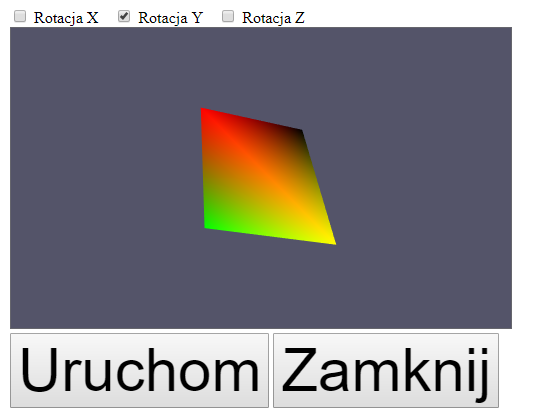
\includegraphics[width=0.6\textwidth,height=8cm]{czworoscian.png}
      \caption{Obracający się czworościan}
      \label{fig:zrzut1}
    \end{figure}

    \begin{figure}[h!]
      \centering
      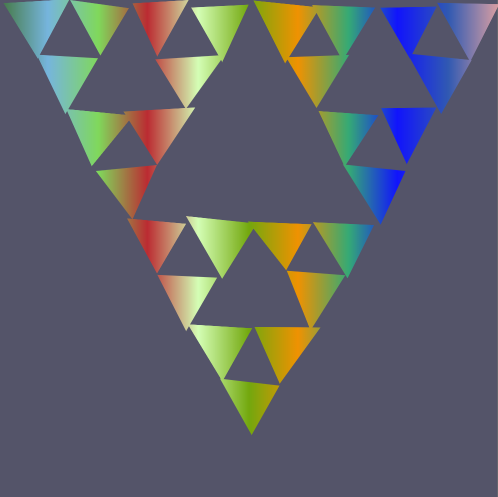
\includegraphics[width=0.6\textwidth,height=8cm]{fraktal1.png}
      \caption{Fraktal. var najwyzszyPoziom = 3, var perturbance = 20}
      \label{fig:zrzut1}
    \end{figure}

    \begin{figure}[h!]
      \centering
      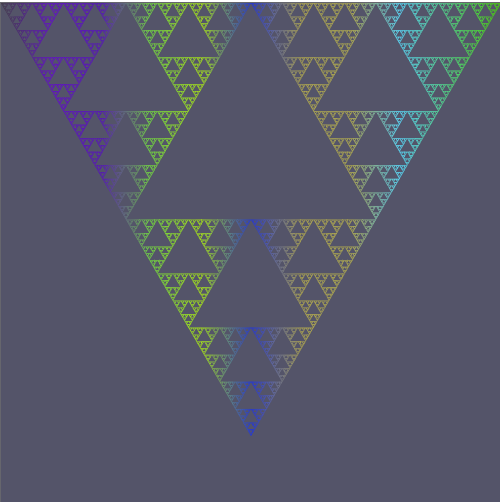
\includegraphics[width=0.6\textwidth,height=8cm]{fraktal2.png}
      \caption{Fraktal. var najwyzszyPoziom = 10, var perturbance = 0}
      \label{fig:zrzut1}
    \end{figure}


\end{document}